% lualatex statestikz-3.tex
% pdf2svg statestikz-3.pdf statestikz-3.svg

\documentclass[border=2bp, tikz]{standalone}
\usepackage{tikz}

\usetikzlibrary{calc,trees,matrix,positioning,chains,fit,intersections}
\usetikzlibrary{arrows,shapes.arrows,shapes.geometric,shapes.multipart,shapes.symbols}
\tikzset{
   state/.style={ rectangle, draw=black, thick, minimum height=1.66em, text centered, rounded corners=3pt},
   error state/.style={ rectangle, double, draw=black, semithick, minimum height=1.66em, text centered, rounded corners=3pt},
   off state/.style={ ellipse, double, draw=black, semithick, minimum height=1.66em, text centered, rounded corners=3pt},
   partial state/.style={ellipse, double, draw=black, semithick, minimum height=1.66em, text centered, rounded corners=3pt},
   branch/.style={ fill, shape=circle, minimum size=3pt, inner sep=0pt},
   cross line/.style={preaction={draw=white, -, shorten >=3pt, shorten <=3pt, line width=2pt}},
   >=latex
}
\usepackage{fontspec}
\setmainfont[UprightFont={Petrona-Light.ttf},
             BoldFont={Petrona-Medium.ttf},
             ItalicFont={Petrona-LightItalic.ttf},
             BoldItalicFont={Petrona-MediumItalic.ttf},
            ]{Petrona-Light.ttf}

\begin{document}
\begingroup
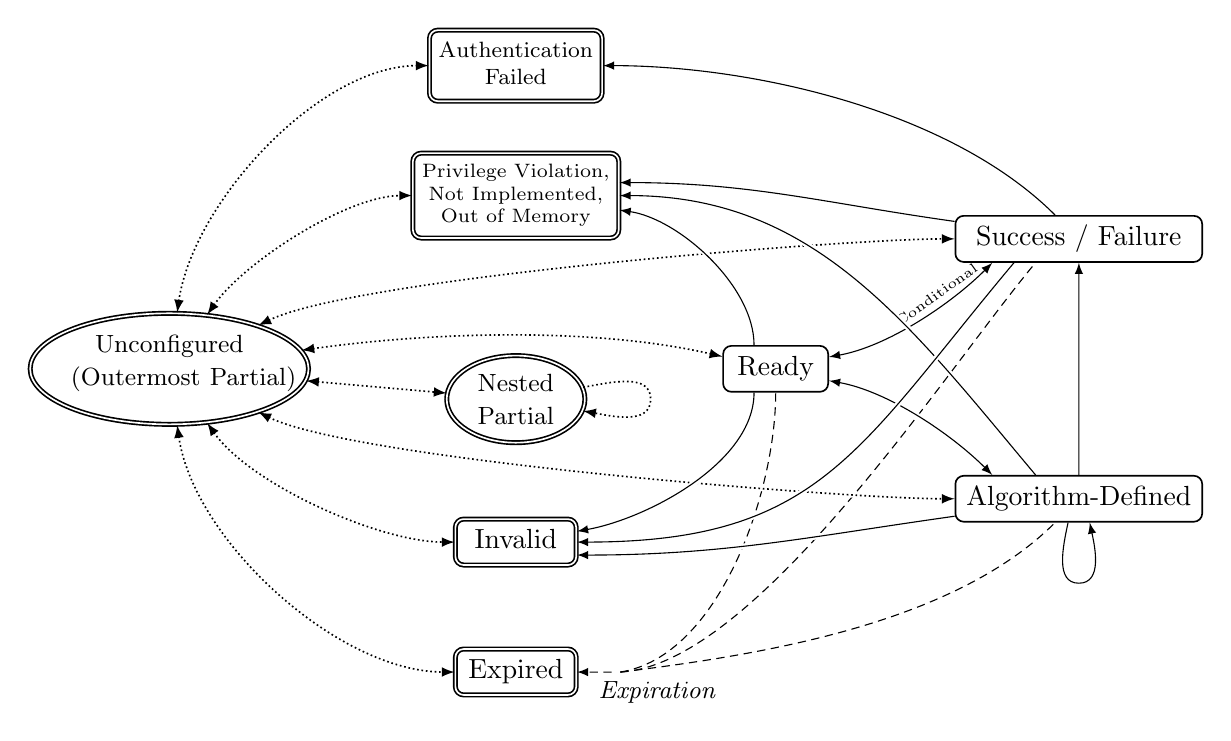
\begin{tikzpicture}[scale=1.1]

  \node[off state,text width=2.5cm,minimum height=1.41cm,inner sep=0pt] at (-4.00,0)  (off) {\small\smash{Unconfigured} \hbox{\smash{(}Outermost Partial\smash{)}~}};

  \node[partial state,text width=1.1cm,inner sep=2pt] at (0,-0.35) (nested partial)  {\small Nested Partial};

  \node[error state, text width=1.3cm] at (0,-2)   (invalidated)    {Invalid\vphantom{g}};
  \node[error state] at (0,2)                      (various errors) {\scriptsize\begin{tabular}{@{}c@{}}Privilege Violation,\\Not Implemented,\\Out of Memory\end{tabular}};
  \node[error state] at (0,3.5)                    (authfail)       {\footnotesize\begin{tabular}{@{}c@{}}Authentication\\Failed\end{tabular}};
  \node[error state, text width=1.3cm] at (0,-3.5) (expired)        {Expired};

  \node[coordinate] at ($(expired.east)+(0.5,0)$)  (before expired) {};

  \node[state, semithick, text width=1.1cm] at (3,0)      (ready)             {Ready\vphantom{g}};
  \node[state, semithick, text width=2.9cm] at (6.5,-1.5) (algorithm defined) {Algorithm-Defined};
  \node[state, semithick, text width=2.9cm] at (6.5,1.5)  (success failure)   {Success / Failure};
  \node[below right=0mm and -4mm of before expired]       (ignore)            {\small\textit{Expiration}};

  \draw[-,densely dashed]   (before expired) to[out=9,in=270,looseness=0.8] (ready);
  \draw[-,densely dashed]   (before expired) to[out=7,in=225,looseness=0.8] (algorithm defined);
  \draw[-,densely dashed]   (before expired) to[out=3,in=230,looseness=0.6] ($(success failure.south)+(-0.501,0)$);
  \draw[->,densely dashed]  ($(before expired)+(-0.1,0)$) -- (expired);

  \draw[<->,semithick,densely dotted] (off) -- (nested partial);

  %% Loop
  \draw[->,semithick,densely dotted] (nested partial) to[out=10,in=90] ($(nested partial.east)+(0.75,0)$) to[out=270,in=-10] (nested partial);

  \draw[<->,semithick,densely dotted] (off) to[out=82,in=180,looseness=0.8]  (authfail);
  \draw[<->,semithick,densely dotted] (off) to[out=55,in=180,looseness=0.7]  (various errors);
  \draw[<->,semithick,densely dotted] (off) to[out=-55,in=180,looseness=0.7] (invalidated);
  \draw[<->,semithick,densely dotted] (off) to[out=-82,in=180,looseness=0.8] (expired);

  %% Loop
  \draw[->] ($(algorithm defined.south)+(-0.125,0)$) to[out=258,in=180]
    ($(algorithm defined.south)+(0,-0.7)$) to[out=0,in=282] ($(algorithm defined.south)+(0.125,0)$);

  \draw[->,cross line] (algorithm defined) to[out=188,in=0,  looseness=1] ($(invalidated.east)+(0,-0.15)$);

  \draw[<->] ($(success failure.south)+(-1,0)$) to[out=225,in=10,looseness=0.8]   node[pos=0.34, above, sloped, yshift=-1pt] () {\tiny Conditional} ($(ready.east)!0.5!(ready.north east)$);

  \draw[<->,semithick,densely dotted] (off) to[out=8,in=167,looseness=0.8] (ready);
  \draw[<->,semithick,densely dotted, cross line] (off) to[out=-26,in=180,looseness=0.4] (algorithm defined);
  \draw[<->,semithick,densely dotted, cross line] (off) to[out=26,in=180,looseness=0.4] (success failure);

  \draw[->,cross line] ($(algorithm defined.north)+(-0.5,0)$) to[out=130,in=0,looseness=1] ($(various errors.east)+(0,0)$);

  \draw[->,cross line] ($(ready.south)+(-0.25,0)$) to[out=270,in=10,looseness=0.8] (invalidated);
  \draw[->,cross line] ($(ready.north)+(-0.25,0)$) to[out=90,in=-8,looseness=0.8] (various errors);


  \draw[<->,cross line] ($(algorithm defined.north)+(-1,0)$) to[out=135,in=-10,looseness=0.8] ($(ready.east)!0.5!(ready.south east)$);
  \draw[->,cross line] (algorithm defined) -- (success failure);

  \draw[->,cross line] (success failure) to[out=135,in=0,looseness=0.8] (authfail);
  \draw[->,cross line] ($(success failure.south)+(-0.75,0)$) to[out=230,in=0,looseness=1.2] (invalidated);

  \draw[->,cross line] (success failure) to[out=172,in=0, looseness=1] ($(various errors.east)+(0,0.15)$);

\end{tikzpicture}
\endgroup
\end{document}
